\documentclass[12pt]{report} % You can use 'article' or 'book' class as well

\usepackage{graphicx} % For including images
\usepackage{amsmath}
\usepackage{amssymb}
\usepackage{multicol}
\usepackage{pgfplots}
\usepackage{tikz}

\begin{document}

% Title page
\begin{titlepage}
	\centering
	\vspace*{1cm} % Adjusts vertical space for the image
	% Insert your image (use the actual path and filename of your image)
	\includegraphics[width=0.3\textwidth]{../images/KMITL Logo.png} % Adjust width as needed

	\vspace{1cm} % Vertical space after the image
	{\LARGE \textbf{Week 7 Homework}} \\[0.5cm] % Title
	\vspace{0.5cm}
	{\large \textbf{Probability Model and Data Analysis}} \\[0.5cm]
    {\large \textbf{Software Engineering Program,}} \\[0.5cm]
	{\large \textbf{Department of Computer Engineering,}} \\[0.5cm]
	{\large \textbf{School of Engineering, KMITL}} \\[1cm]
    {\Large 67011352 Theepakorn Phayonrat} \\[0.5cm] % Authors (Use \\ the separate authors)
\end{titlepage}

\section*{Homework of Binomial and Poisson RVs}

\subsection*{Binomial RVs:}
\subsection*{Question 1:}

\noindent Flip a fair coin two times. Observe each trial whether head
or tail facing up after the coin lands. Assume that two trials are
independent. The event the head facing up is considered as a success
while the  event of the tail facing up is considered as a failure.
Let $X$ be the number of success. \\

\noindent (1) Find and sketch the PMF of $X$ \\
(2) Find the expected value $E[X]$ \\
(3) Find and sketch the CDF of $X$ \\

\subsection*{Solution}

\noindent To find the Binomial random variable $X$ we need to find
the Bernoulli random variable of each trial. \\

\noindent Let $C$ be the random variable of the success event of
a Bernoulli trial. \\
\[
P_C[c] =
\begin{cases}
    0.5 & c = 0 \\
    0.5 & c = 1 \\
    0 & otherwise \\
\end{cases}
\]
\noindent After we have got the PMF of the Bernoulli trial, we can find
the Binomial random variable $X$ where the result implies from PMF of
$C$ where $P_C[c = 1]$ is the success event (head facing up) and
$P_C[c = 1]$ is the failure event (tail facing up). \\

\[
P_X[x] =
\begin{cases}
    \binom{2}{x}(P_C[c = 1])^{x}(P_C[c = 0])^{2-x} & x = 0, 1, 2 \\
    0 & otherwise \\
\end{cases}
\]

\newpage

\begin{multicols}{2}
\[
\therefore P_X(x) =
\begin{cases}
0.25 & x = 0, \\
0.5 & x = 1, \\
0.25 & x = 2, \\
1 & \text{otherwise}.
\end{cases}
\]
\columnbreak
\\
\begin{center}
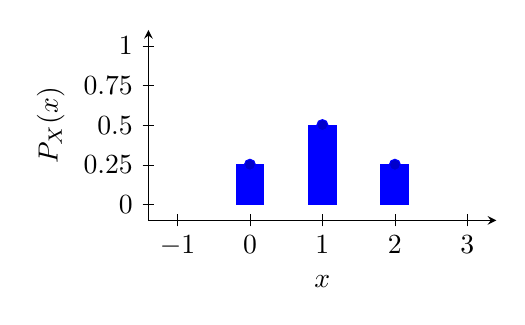
\begin{tikzpicture}
\begin{axis}[
    ymin=0, ymax=1,
    xmin=-1, xmax=3,
    xtick={-1,0,1,2,3},
    ytick={0,0.25,0.5,0.75,1},
    axis lines=left,
    width=6cm,
    height=4cm,
    enlargelimits=0.1,
    ylabel={$P_X(x)$},
    xlabel={$x$},
    tick style={black},
    ymajorgrids=false,
    xmajorgrids=false,
    every axis plot/.append style={ybar, bar width=10pt, black, fill=black}
]
\addplot coordinates {(0,0.25) (1,0.5) (2,0.25)};
\end{axis}
\end{tikzpicture}
\end{center}
\end{multicols}

\noindent $\therefore$ The expected value $E[X] = np = (2)(0.5) = 1$ \\

\noindent After we have got the PMF, we can now find the CDF of the
Binomial random variable $X$. \\

\begin{multicols}{2}
\[
\therefore F_X(x) =
\begin{cases}
0 & x < 0, \\
0.25 & 0 \le x < 1, \\
0.75 & 1 \le x < 2, \\
1 & x \ge 2 \\
\end{cases}
\]
\columnbreak
\\
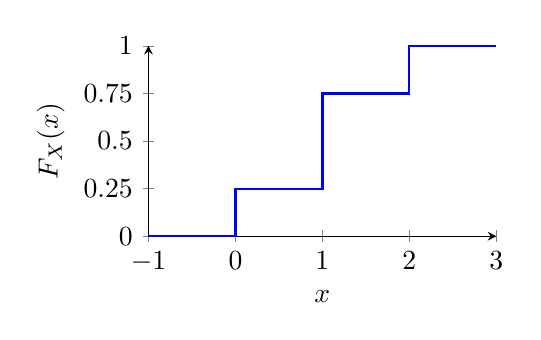
\begin{tikzpicture}
    \begin{axis}[
        width=6cm,
        height=4cm,
        xmin=-1, xmax=3,
        ymin=0, ymax=1,
        axis x line=bottom,
        axis y line=left,
        xlabel={$x$},
        ylabel={$F_X(x)$},
        ytick={0,0.25,0.5,0.75,1},
        xtick={-1,0,1,2,3},
        domain=0:5,
        samples=100,
        no marks,
        clip=false
    ]
    \addplot[blue, thick] coordinates {(-1,0) (0,0) (0,0.25) (1,0.25) (1,0.75) (2,0.75) (2,1) (3,1)};
    \end{axis}
\end{tikzpicture}
\end{multicols}

\newpage

\subsection*{Poisson RVs:}
\subsection*{Question 2:}

\noindent The number of cars pulling into the parking garage every
sixty minutes can be described as a Poisson process. If, on average,
5 cars enter the garage every sixty minutes, what is the probability
that \textit{at most} 1 car will arrive in the next hour?

\subsection*{Solution}

\noindent We all know that 60 minutes equal to 1 hour. \\
$\therefore T = 1$ (Time period is 1 hour) \\
$\therefore \lambda = 5$ (Average rate is 5 cars) \\
$\therefore \alpha = (\lambda)(T) = (5)(1) = 5$ (Poisson random variable) \\
\begin{equation} \notag
\begin{split}
    \therefore P_X[x \le 1] & = \sum_{n=0}^{1} P_X[x = n] \\
                            & =  \sum_{n=0}^{1} \frac{\alpha^{x}e^{-\alpha}}{x!} ; \alpha = 5 \\
                            & = \frac{(5^{0})(e^{-5})}{0!} + \frac{(5^{1})(e^{-5})}{1!} \\
                            & = (5^{0} + 5^{1})(e^{-5}) \\
                            & = (6)(e^{-5}) \\
                            & \approx 0.04043 \\
\end{split}
\end{equation}

\subsection*{Answer}

\noindent $\therefore$ The approximate probability that at most 1 car will
arrive in the next hour is $0.04043$ \\

\end{document}
